\documentclass{article}

\usepackage{inputenc}
\usepackage{csquotes}
\usepackage[a4paper, total={6in, 10in}]{geometry}
\usepackage{hyperref}
\usepackage{amsmath,amssymb}
\usepackage{graphicx}
\usepackage{indentfirst}
\usepackage{caption}
\usepackage{subcaption}
\usepackage[
singlelinecheck=false % <-- important
]{caption}
\usepackage{float}
\usepackage{booktabs}
\begin{document}

   \begin{figure}[H]
       \centering
       \caption{\textbf{Implied treatment effects}}
       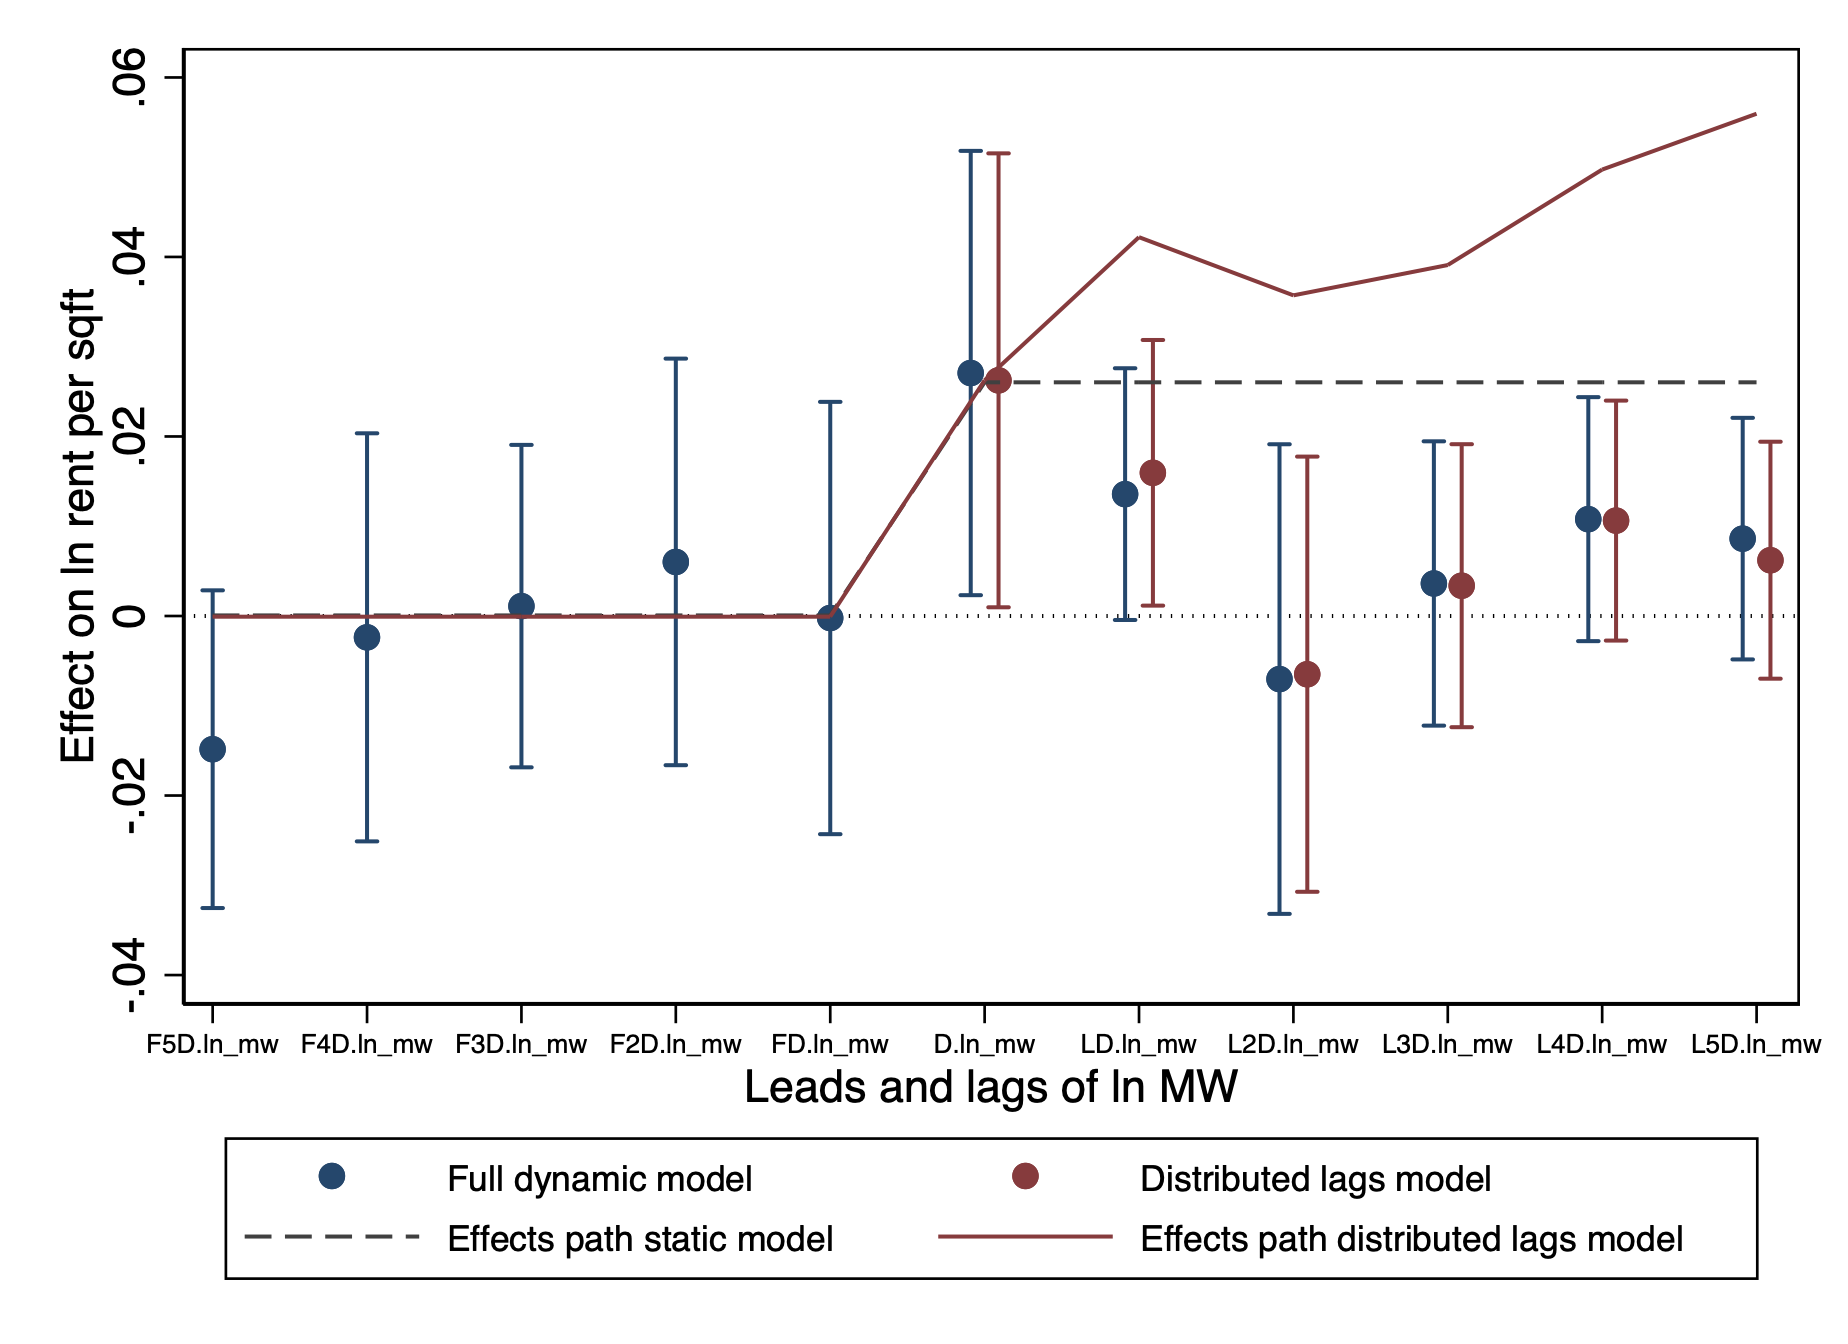
\includegraphics[width = \textwidth]{../analysis/first_differences/output/fd_models}
       \label{fig: implied_paths}
  \end{figure}

\begin{table}[h!]
\caption{\textbf{First-difference panel specifications}}
    \centering
  \begin{subtable}[t]{\linewidth}
          \caption*{\textbf{Panel A: Two-way fixed effects}}

    \centering
    \resizebox{\textwidth}{!}{
    \vspace{0pt}    
    {
\def\sym#1{\ifmmode^{#1}\else\(^{#1}\)\fi}
\begin{tabular}{l*{8}{c}}
\hline\hline
          &\multicolumn{1}{c}{(1)}&\multicolumn{1}{c}{(2)}&\multicolumn{1}{c}{(3)}&\multicolumn{1}{c}{(4)}&\multicolumn{1}{c}{(5)}&\multicolumn{1}{c}{(6)}&\multicolumn{1}{c}{(7)}&\multicolumn{1}{c}{(8)}\\
          &\multicolumn{1}{c}{DiD}&\multicolumn{1}{c}{Distributed leads and lags}&\multicolumn{1}{c}{Distributed Lags}&\multicolumn{1}{c}{AB distributed leads and lags}&\multicolumn{1}{c}{AB distributed lags}&\multicolumn{1}{c}{est6}&\multicolumn{1}{c}{est7}&\multicolumn{1}{c}{est8}\\
\hline
\Delta ln(MW)_{t-5}&                  &  -0.0146         &                  &  -0.0159         &  -0.0134         &                  &  -0.0167         &                  \\
          &                  &(0.00910)         &                  &(0.00991)         &(0.00910)         &                  & (0.0155)         &                  \\
[1em]
\Delta ln(MW)_{t-4}&                  & -0.00232         &                  & -0.00576         &  0.00494         &                  & -0.00886         &                  \\
          &                  & (0.0116)         &                  & (0.0129)         & (0.0105)         &                  & (0.0347)         &                  \\
[1em]
\Delta ln(MW)_{t-3}&                  &  0.00137         &                  &  0.00100         &  0.00222         &                  & 0.000503         &                  \\
          &                  &(0.00931)         &                  & (0.0106)         &(0.00918)         &                  & (0.0152)         &                  \\
[1em]
\Delta ln(MW)_{t-2}&                  &  0.00608         &                  &  0.00625         &  0.00581         &                  &  0.00647         &                  \\
          &                  & (0.0115)         &                  & (0.0107)         & (0.0139)         &                  & (0.0102)         &                  \\
[1em]
\Delta ln(MW)_{t-1}&                  &-0.000280         &                  & -0.00141         & -0.00531         &                  &-0.000132         &                  \\
          &                  & (0.0123)         &                  &(0.00995)         & (0.0151)         &                  & (0.0154)         &                  \\
[1em]
\Delta ln(MW)_{t}&   0.0259\sym{*}  &   0.0270\sym{**} &   0.0261\sym{*}  &   0.0269\sym{**} &   0.0294\sym{*}  &   0.0288\sym{*}  &   0.0267\sym{**} &   0.0256\sym{**} \\
          & (0.0129)         & (0.0127)         & (0.0129)         & (0.0111)         & (0.0157)         & (0.0160)         & (0.0104)         & (0.0106)         \\
[1em]
\Delta ln(MW)_{t+1}&                  &   0.0136\sym{*}  &   0.0161\sym{**} &   0.0205\sym{**} & 0.000887         &  0.00401         &   0.0267         &   0.0304         \\
          &                  &(0.00715)         &(0.00750)         &(0.00860)         &(0.00733)         &(0.00788)         & (0.0514)         & (0.0536)         \\
[1em]
\Delta ln(MW)_{t+2}&                  & -0.00702         & -0.00673         & -0.00389         &  -0.0131         &  -0.0142         & -0.00102         &  0.00170         \\
          &                  & (0.0133)         & (0.0125)         & (0.0138)         & (0.0128)         & (0.0120)         & (0.0286)         & (0.0354)         \\
[1em]
\Delta ln(MW)_{t+3}&                  &  0.00364         &  0.00392         &  0.00211         &  0.00651         &  0.00692         & 0.000616         & 0.000316         \\
          &                  &(0.00808)         &(0.00799)         &(0.00972)         &(0.00798)         &(0.00764)         & (0.0158)         & (0.0173)         \\
[1em]
\Delta ln(MW)_{t+4}&                  &   0.0108         &   0.0105         &   0.0112         &  0.00897         &  0.00850         &   0.0120         &   0.0122         \\
          &                  &(0.00693)         &(0.00684)         &(0.00737)         &(0.00736)         &(0.00737)         & (0.0108)         & (0.0119)         \\
[1em]
\Delta ln(MW)_{t+5}&                  &  0.00862         &  0.00637         &   0.0102         &  0.00384         &  0.00163         &   0.0124         &   0.0112         \\
          &                  &(0.00686)         &(0.00675)         &(0.00655)         &(0.00878)         &(0.00870)         & (0.0160)         & (0.0174)         \\
[1em]
\Delta ln(y)_{t-1}&                  &                  &                  &   -0.240\sym{***}&    0.421\sym{***}&    0.436\sym{***}&   -0.451         &   -0.531         \\
          &                  &                  &                  &(0.00646)         & (0.0238)         & (0.0231)         &  (1.634)         &  (1.812)         \\
\hline
Observations& 1.12e+05         & 1.06e+05         & 1.12e+05         & 1.05e+05         & 1.04e+05         & 1.10e+05         & 1.05e+05         & 1.11e+05         \\
\hline\hline
\end{tabular}
}

    }
    \end{subtable}
      
  \begin{subtable}[t]{\linewidth}
      \caption*{\textbf{Panel B: Two-way fixed effects with zipcode specific linear trends}}
    \centering
     \resizebox{\textwidth}{!}{
    \vspace{0pt}    
    {
\def\sym#1{\ifmmode^{#1}\else\(^{#1}\)\fi}
\begin{tabular}{l*{5}{c}}
\hline\hline
          &\multicolumn{1}{c}{(1)}&\multicolumn{1}{c}{(2)}&\multicolumn{1}{c}{(3)}&\multicolumn{1}{c}{(4)}&\multicolumn{1}{c}{(5)}\\
          &\multicolumn{1}{c}{DiD}&\multicolumn{1}{c}{Distributed leads and lags}&\multicolumn{1}{c}{Distributed Lags}&\multicolumn{1}{c}{AB distributed leads and lags}&\multicolumn{1}{c}{AB distributed lags}\\
\hline
\Delta ln(MW)\_{t-2}&                  &  0.00616         &                  &  0.00623         &                  \\
          &                  & (0.0125)         &                  & (0.0114)         &                  \\
[1em]
\Delta ln(MW)\_{t-1}&                  &-0.000917         &                  & -0.00225         &                  \\
          &                  & (0.0130)         &                  & (0.0108)         &                  \\
[1em]
\Delta ln(MW)\_{t}&   0.0257\sym{**} &   0.0270\sym{**} &   0.0261\sym{**} &   0.0270\sym{**} &   0.0262\sym{**} \\
          & (0.0120)         & (0.0122)         & (0.0124)         & (0.0105)         & (0.0106)         \\
[1em]
\Delta ln(MW)\_{t+1}&                  &   0.0161\sym{*}  &   0.0155\sym{*}  &   0.0226\sym{**} &   0.0221\sym{**} \\
          &                  &(0.00842)         &(0.00811)         &(0.00949)         &(0.00925)         \\
[1em]
\Delta ln(MW)\_{t+2}&                  & -0.00720         & -0.00704         & -0.00332         & -0.00316         \\
          &                  & (0.0125)         & (0.0126)         & (0.0130)         & (0.0130)         \\
[1em]
\Delta ln(y)\_{t-1}&                  &                  &                  &   -0.240\sym{***}&   -0.239\sym{***}\\
          &                  &                  &                  &(0.00638)         &(0.00619)         \\
\hline
R-squared &    0.024         &    0.024         &    0.024         &    0.081         &    0.080         \\
Observations&   112232         &   109940         &   112226         &   108803         &   111089         \\
\hline\hline
\end{tabular}
}

    }
    \end{subtable}
    
  \begin{subtable}[t]{\linewidth}
      \caption*{\textbf{Panel C: Two-way fixed effects with zipcode specific quadratic trends}}

    \centering
    \resizebox{\textwidth}{!}{
    \vspace{0pt}    
    {
\def\sym#1{\ifmmode^{#1}\else\(^{#1}\)\fi}
\begin{tabular}{l*{5}{c}}
\hline\hline
          &\multicolumn{1}{c}{(1)}&\multicolumn{1}{c}{(2)}&\multicolumn{1}{c}{(3)}&\multicolumn{1}{c}{(4)}&\multicolumn{1}{c}{(5)}\\
          &\multicolumn{1}{c}{DiD}&\multicolumn{1}{c}{Distributed leads and lags}&\multicolumn{1}{c}{Distributed Lags}&\multicolumn{1}{c}{AB distributed leads and lags}&\multicolumn{1}{c}{AB distributed lags}\\
\hline
\Delta ln(MW)\_{t-2}&                  &  0.00616         &                  &  0.00621         &                  \\
          &                  & (0.0124)         &                  & (0.0111)         &                  \\
[1em]
\Delta ln(MW)\_{t-1}&                  & -0.00130         &                  & -0.00248         &                  \\
          &                  & (0.0138)         &                  & (0.0120)         &                  \\
[1em]
\Delta ln(MW)\_{t}&   0.0255\sym{**} &   0.0267\sym{**} &   0.0259\sym{**} &   0.0267\sym{**} &   0.0261\sym{**} \\
          & (0.0117)         & (0.0118)         & (0.0121)         & (0.0102)         & (0.0102)         \\
[1em]
\Delta ln(MW)\_{t+1}&                  &   0.0160\sym{*}  &   0.0152\sym{*}  &   0.0226\sym{**} &   0.0219\sym{**} \\
          &                  &(0.00901)         &(0.00851)         &(0.00992)         &(0.00951)         \\
[1em]
\Delta ln(MW)\_{t+2}&                  & -0.00720         & -0.00726         & -0.00321         & -0.00323         \\
          &                  & (0.0120)         & (0.0122)         & (0.0124)         & (0.0125)         \\
[1em]
\Delta ln(y)\_{t-1}&                  &                  &                  &   -0.243\sym{***}&   -0.242\sym{***}\\
          &                  &                  &                  &(0.00641)         &(0.00620)         \\
\hline
R-squared &    0.026         &    0.027         &    0.026         &    0.085         &    0.084         \\
Observations&   112232         &   109940         &   112226         &   108803         &   111089         \\
\hline\hline
\end{tabular}
}

    }
    \end{subtable}
   \end{table}
   
\end{document}